
\documentclass[a4paper]{article} %
\usepackage{graphicx,amssymb} %

\textwidth=15cm \hoffset=-1.2cm %
\textheight=25cm \voffset=-2cm %

\pagestyle{empty} %

\date{} %

\def\keywords#1{\begin{center}{\bf Keywords}\\{#1}\end{center}} %

\def\titulo#1{\title{#1}} %
\def\autores#1{\author{#1}} %

% Please, do not change any of the above lines








\begin{document}

% Type down your paper title
\titulo{Envelope computation in dynamic geometry systems}

% Authors
\autores{Francisco Botana \\ %
       Universidad de Vigo (Spain) \\ \\ % Affiliation 1
       Tomas Recio \\ % If any other author with different Affilation
       Universidad de Cantabria (Spain) \\ \\ % Affiliation 2 (if needed)
       % New author \\
       % New affiliation \\
       % Add authors and affiliation as needed
       \tt{fbotana@uvigo.es} % Only one corresponding e-mail
       }%


\maketitle

\thispagestyle{empty}



% The abstract

\begin{abstract}
Considerable attention has been given to the computation of geometric loci in dynamic geometry, from both graphical and equational viewpoints. Recent work has established a rigourous approach to the last issue, solving the subject for the algebraic realm. 
Nevertheless, although the automatic computation of envelopes could be seen as an analogous problem, there are cases where unexpected difficulties emerge.

In this talk we review the state of the art of common dynamic geometry software when dealing with envelopes. Despite their maturity in other subjects, envelopes are generally considered as purely graphic objects in such environments, without any analytic knowledge about them.

We also describe a data structure needed to cope with envelopes in dynamic geometry, and a Sage program able to compute usual envelopes in an efficient way. Finally, in order to show the complexities of such computations, we discuss the envelope of a simple family of ellipses. The search for such envelope will illustrate two facts:
\begin{enumerate}
 \item There is no general agreement between dynamic geometry developers about the definition of envelope, and
 \item Currently, the simple application of computer algebra techniques is not enough to automatically solve the problem. 
\end{enumerate}



\end{abstract}

\keywords{Dynamic Geometry, Automated Deduction in Geometry, Envelope Computation} % Write down at least 3 Keywords






\section{Introduction}
Given a family of curves $C_\alpha: F(x,y,\alpha)=0$, its {\it envelope} or {\it discriminant} is defined \cite{BruceGiblin} as the set
$$\mathcal{D}=\{(x,y) \in \mathbb{R}^2:{\rm  there}\: {\rm exists} \: \alpha \in \mathbb{R}\: {\rm with}\: F(x,y,\alpha)=\frac{\partial F}{\partial \alpha}=0\}.$$
Other definitions coexist with this one, for instance
\begin{itemize}
 \item The envelope $E_1$ is the limit of intersections of nearby curves $C_\alpha$.
 \item The envelope $E_2$ is a curve tangent to the $C_\alpha$.
 \item The envelope $E_3$ is the boundary of the region filled by the curves $C_\alpha$.
\end{itemize}
where it can be proved that $E_i \subset \mathcal{D}, i=1,\dots,3$. While $E_1$ seems to be the interpretation of envelopes given by Lagrange to singular solutions 
of differential equations (see \cite{Yates}), $E_3$ and, to a lesser extent, $E_2$ are behind the intuitive notion of envelope used in dynamic geometry environments. 
Since these systems are mostly based on a graphical simulation of geometry, their ability to trace geometrc elements is succesfully used to suggest envelopes. 
Consider, for instance, the family of ellipses with foci in $A(4,0)$, $B(0,\alpha)$ (a semifree point on the $y$ axis) and major axis with length 5. 

\begin{figure}[htp]
\begin{center}
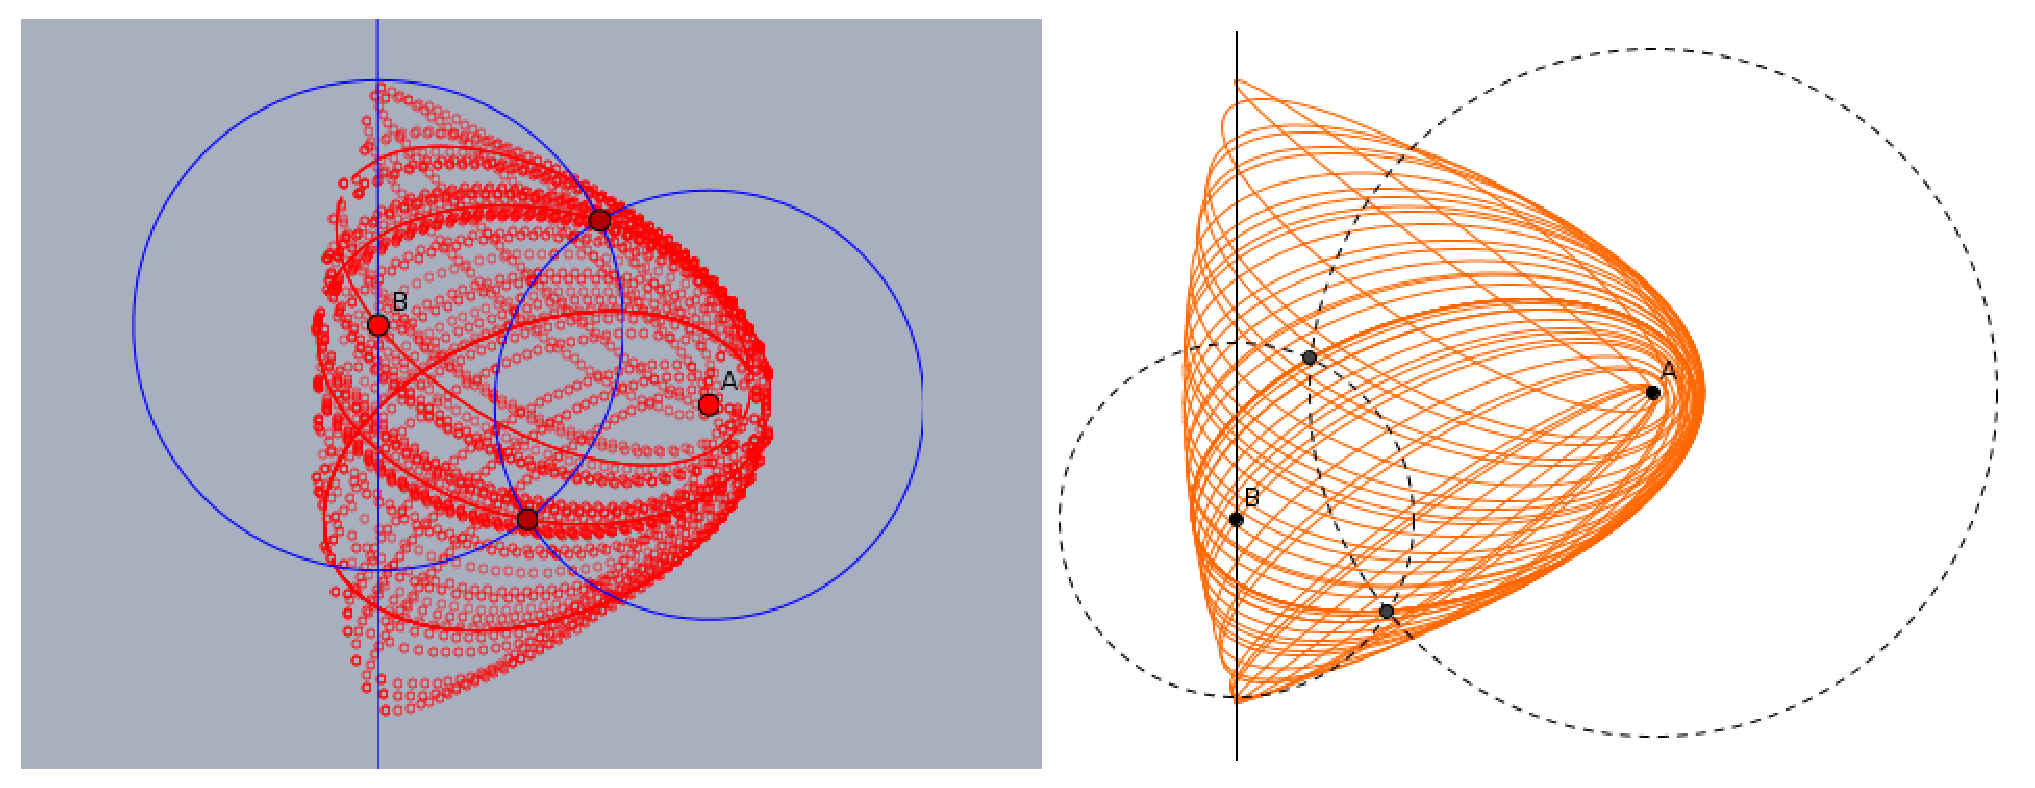
\includegraphics[width=12cm]{fig0.eps}
\caption{A family of ellipses obtained as loci (left: Cinderella, right: GeoGebra) is traced to suggest its envelope.}
\end{center}
\end{figure}

If a user activates the trace option for the variable ellipse and moves the point $B$ along its path, a plane region is drawn (Figure 1), the border being the sought envelope, 
if the third alternative definition is used. Nevertheless, as usual in dynamic geometry, the user gets a cursory knowledge: no result about the type of curves defining the 
border is returned. Even worse, consider a region with holes, or without border. In this last case, the strategy of tracing the family curves could mislead an inexperienced 
user, as exemplified by searching for the envelope of straight lines passing through the origin.

It should be noted that although there exist a well known dynamic geometry software, Cabri, able to compute equations for constructed objects, its numerical approach is 
not robust and does not return any result for the above family.

\section{A parametric approach for the envelope problem}
Several authors (see, for instance, \cite{Botana,Roanes}) have proposed extending the data structure of dynamic geometry systems to include what can be called a 
{\it parametric description} of constructions. This description involves keeping the relation between primitive and dependent objects in such a way that any assignment of the 
free variables (i.e., coordinates of basic points and equations of other initial objects) would trigger the {\it actual} computation of dependent objects.

Using the Sage library in \cite{SageLib}, a generic ellipse of the family could be defined by
\begin{verbatim}
FreePoint('A',4,0)
FreePoint('P1',0,0)
FreePoint('P2',0,1)
Line('y','P1','P2')
PointOnObject('B','y')
FreePoint('M',2,2)
FreePoint('N',2,7)
Line('MN','M','N')
PointOnObject('P','MN')
Circle('c1','A','M','P')
Circle('c2','B','N','P')
IntersectionObjectObject('X','c1','c2')
Locus2('loc','X','B','P')
\end{verbatim}
\noindent where the \verb+Locus2+ function contains a parametric representation of the ellipse. That is, its algebraic description is not a function in two variables, but it also 
contains the parameter of the variable point $B$. The polynomial of the family is
$$4y^2\alpha^2 - 4y\alpha^3 - 36x^2 - 100y^2 + \alpha^4 - 32xy\alpha + 16x\alpha^2 + 164y\alpha - 82\alpha^2 + 144x + 81,$$
and one could then use the first definition of envelope to find its equation. The elimination of $\alpha$ returns
$$x^2y^4 + y^6 - 16x^3y^2 - 24xy^4 - 36x^4 + 74x^2y^2 - 2y^4 + 432x^3 + 32xy^2 - 1647x^2 - 207y^2 + 1656x + 1296,$$
and, after factoring,
$$(y^2 - 18x - 9)(y^2 + 2x - 9)(x^2 + y^2 -8x + 16).$$
\noindent Thus, the border of the family of elipses consists of (part) of the above parabolas. Nevertheless,...

\section{Things are not so simple}
There is a third factor in the expression of the discriminant that is not part of the border. In fact, this factor is the focus $A$! While understanding why this point appears as 
part of the discriminant has not been a trivial task (as will be illustrated in the talk), we note that asking, for instance, Wolfram$|$Alpha, should give a hint about 
what is happening (Figure 2).

\begin{figure}[htp]
\begin{center}
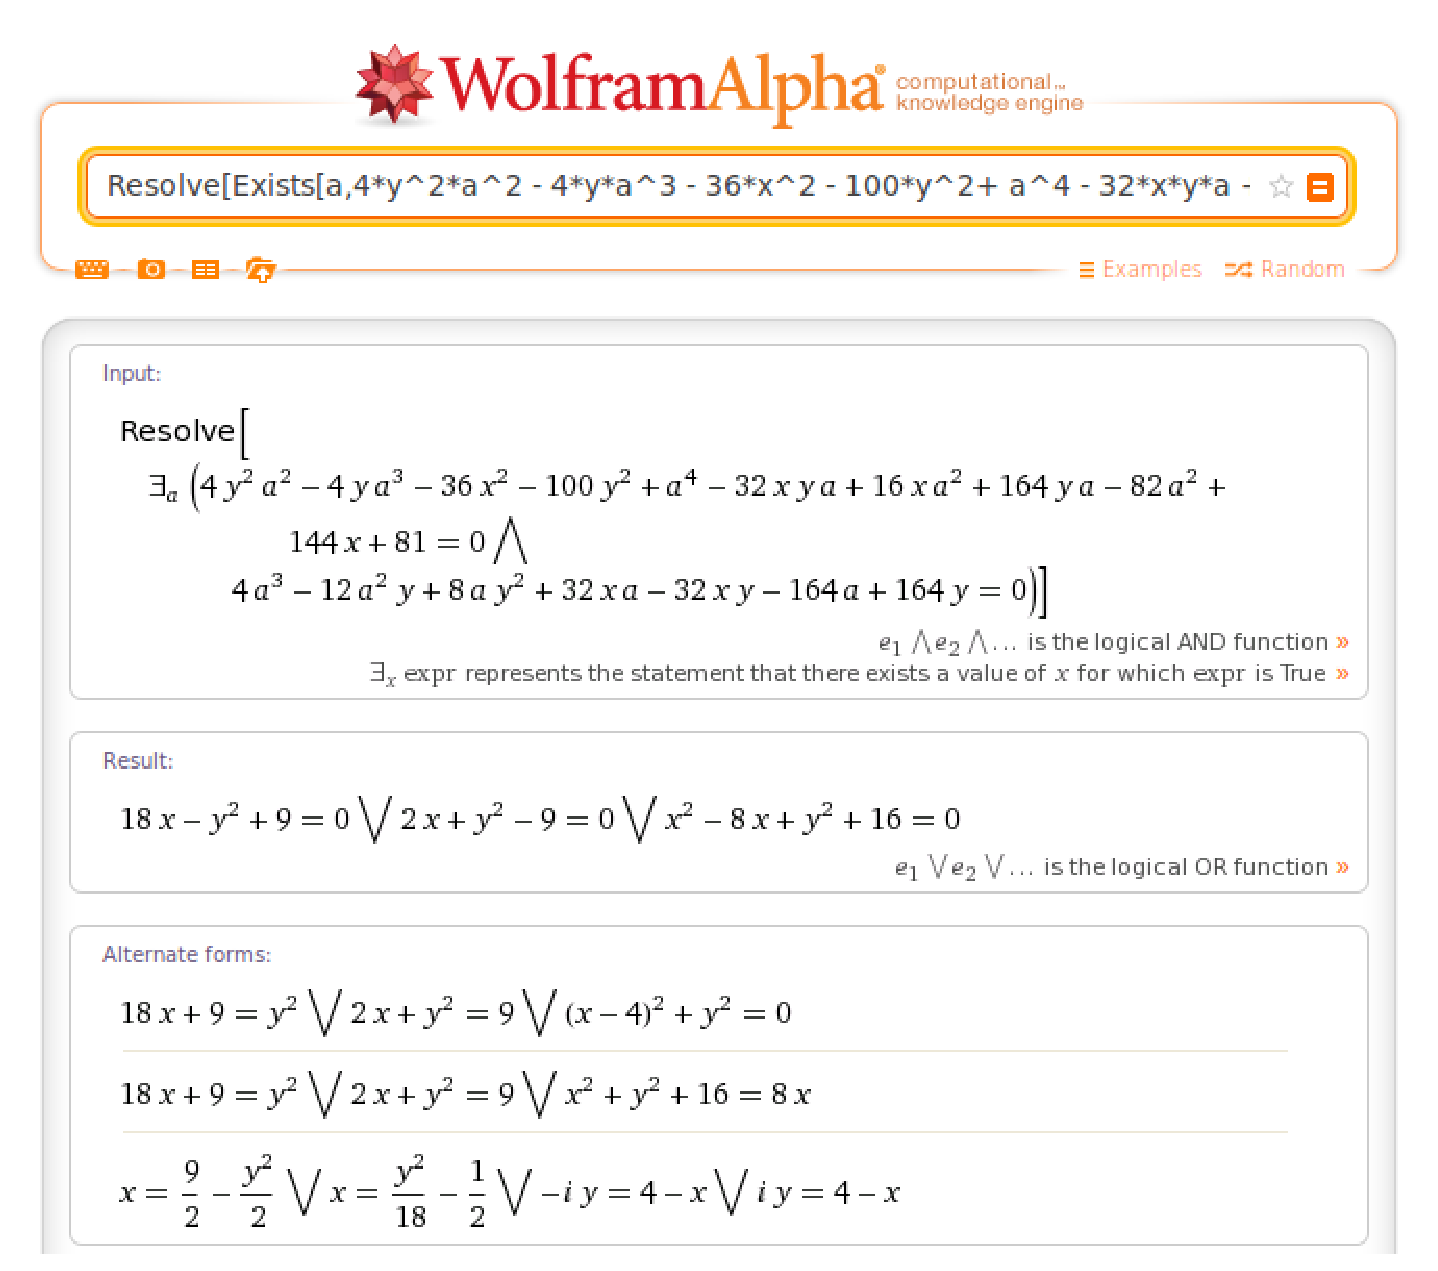
\includegraphics[width=12cm]{wa.eps}
\caption{Wolfram$|$Alpha suggests that point $A(4,0)$ comes from complex components of the envelope.}
\end{center}
\end{figure} 

The moral of this short note is the need of a most rigorous approach when applying algebraic methods valid in $\mathbb{C}$ to misunderstood situations. Here, the family of 
ellipses is semialgebraic. Thus, automated approaches relying on complex approaches should used with caution!

\section*{Acknowledgement}
The authors have been partially supported by the Spanish ``Ministerio de Econom{\'\i}a y Competitividad'' and the ``European Regional Development Fund'' (FEDER),  under 
the project MTM2011--25816--C02--02.
  
%\section*{Referencias}
\begin{thebibliography}{9}
\bibitem{BruceGiblin}J.W. Bruce, P.J. Giblin, Curves and Singularities. Cambridge: Cambridge University Press, 1984.
\bibitem{Yates}R.C. Yates, A Handbook on Curves and Their Properties. Ann Arbor, MI: J. W. Edwards, 1952.
\bibitem{Botana}F. Botana, On the Parametric Representation of Dynamic Geometry Constructions, in B. Murgante {\it et al.} (Eds.), Computational Science and Its Applications -- 
ICCSA 2011, Springer LNCS 6785, pp. 342--352, 2011.
\bibitem{Roanes}E. Roanes-Lozano, E. Roanes-Mac\'{i}as, M. Villar, A bridge between dynamic geometry and computer algebra. Mathematical and Computer Modelling 37, pp. 
1005--1028, 2003.
\bibitem{SageLib}Sage Automated Discovery library, http://webs.uvigo.es/fbotana/AutDiscLib.txt.
\end{thebibliography}

\end{document}
